\usetikzlibrary{arrows.meta}
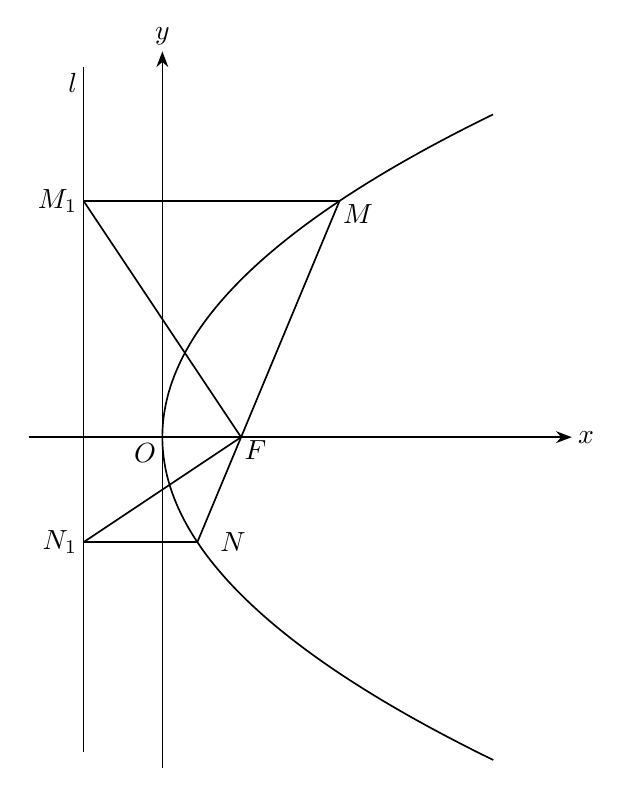
\begin{tikzpicture}[x=1cm,y=1cm,line width=.6pt,>={Stealth},font=\normalsize]
\coordinate (O) at (0,0);
\coordinate (F) at (1,0);
\coordinate (M) at (2.25,3);
\coordinate (N) at (0.444444,-1.333333);
\coordinate (M1) at (-1,3);
\coordinate (N1) at (-1,-1.333333);
\draw[->] (-1.7,0) -- (5.2,0) node[right,inner sep=0pt,xshift=2pt] {$x$};
\draw[->] (0,-4.2) -- (0,4.9) node[above,inner sep=0pt,yshift=2pt] {$y$};
\draw[domain=-4.1:4.1,samples=161,smooth] plot ({(\x*\x)/4},{\x});
\draw (-1,-4.0) -- (-1,4.7);
\draw (M1) -- (M);
\draw (N1) -- (N);
\draw (M1) -- (F);
\draw (N1) -- (F);
\draw (M) -- (N);
\node[left,inner sep=0pt,xshift=-2pt] at (M1) {$M_1$};
\node[left,inner sep=0pt,xshift=-2pt] at (N1) {$N_1$};
\node[below right,inner sep=0pt,xshift=1pt,yshift=-1pt] at (M) {$M$};
\node[right,inner sep=0pt,xshift=8pt] at (N) {$N$};
\node[below right,inner sep=0pt,xshift=1pt,yshift=-1pt] at (F) {$F$};
\node[below left,inner sep=0pt,xshift=-2pt,yshift=-2pt] at (O) {$O$};
\node[left,inner sep=0pt,xshift=-2pt] at (-1,4.5) {$l$};
\end{tikzpicture}
